\exercises

%%%%%%%%%%%%%%%%%%%%%%%%%%%%%%%%%%%%%%%%%%%%%%%%%%%%%%%%%%%%%%%%%%%%%%%%
% Class types
%
\begin{exercise}{class-types1}
What are the class types for the following classes?

\begin{enumerate}
\item

\begin{ocamllisting}
class c1 =
object
   val x = 1
   method get = x
end
\end{ocamllisting}

\begin{answer}\ifanswers
\begin{ocamllisting}
class c1 :
object
   val x : int
   method get : int
end
\end{ocamllisting}
\fi\end{answer}

\item

\begin{ocamllisting}
class c2 =
object
   method copy = {< >}
end
\end{ocamllisting}

\begin{answer}\ifanswers
\begin{ocamllisting}
class c2 :
object ('self)
   method copy : 'self
end
\end{ocamllisting}
\fi\end{answer}

\item

\begin{ocamllisting}
class c3 y =
object (self1)
   method f x =
      object (self2)
         val x = x
         method h = self1#g + x
      end
   method g = y
end
\end{ocamllisting}

\begin{answer}\ifanswers
\begin{ocamllisting}
class c3 : int ->
object
   method f : int -> < h : int >
   method g : int
end
\end{ocamllisting}
\fi\end{answer}

\item

\begin{ocamllisting}
class c4 =
object (self : < x : int; .. > as 'self)
   method private x = 1
end
\end{ocamllisting}

\begin{answer}\ifanswers
The type constraint removes the private status of the method \hbox{\lstinline/x/}.
\begin{ocamllisting}
class c4 :
object 
   method x : int
end
\end{ocamllisting}
\fi\end{answer}
\end{enumerate}
\end{exercise}

%%%%%%%%%%%%%%%%%%%%%%%%%%%%%%%%%%%%%%%%%%%%%%%%%%%%%%%%%%%%%%%%%%%%%%%%
% Initializer order
%
\begin{exercise}{classes-initializer-order}
What does the following program print out?

\begin{ocaml}
class a (i : int) =
let () = print_string "A let\n" in
object
   initializer print_string "A init\n"
end;;

class b (i : int) =
let () = print_string "B let\n" in
object
   inherit a i
   initializer print_string "B init\n"
end;;

new b 0;;
\end{ocaml}

\begin{answer}\ifanswers
The order of the let-expressions and initializers follows the textual order.
Class \hbox{\lstinline/a/} is nested within \hbox{\lstinline/b/}, but before \hbox{\lstinline/b/}'s initializer.
The sequence is the following.

\begin{ocaml}
B let
A let
A init
B init
\end{ocaml}
\fi\end{answer}
\end{exercise}

%%%%%%%%%%%%%%%%%%%%%%%%%%%%%%%%%%%%%%%%%%%%%%%%%%%%%%%%%%%%%%%%%%%%%%%%
% Inverted inheritance
%
\begin{exercise}{classes1}
Normally, we would consider a square to be a subtype of rectangle.
Consider the following class \hbox{\lstinline/square/} that implements a square,

\begin{ocaml}
class square x y w =
object
   val x = x
   val y = y
   method area = w * w
   method draw = Graphics.fill_rect x y w w
   method move dx dy = {< x = x + dx; y = y + dy >}
end
\end{ocaml}
%
Write a class \hbox{\lstinline/rectangle/} that implements a rectangle by inheriting from \hbox{\lstinline/square/}.
Is it appropriate to say that a \hbox{\lstinline/rectangle/} is a \hbox{\lstinline/square/}?

\begin{answer}\ifanswers
The class \hbox{\lstinline/rectangle/} adds a new dimension \hbox{\lstinline/h/}.
\begin{ocaml}
class rectangle x y w h =
object
   inherit square
   method area = w * h
   method draw = Graphics.fill_rect x y w h
end
\end{ocaml}
%
It is appropriate to say that the \emph{representation} of a rectangle includes the representation
of a square.  The is-a relationships in the program are defined by the programmer.  They don't have
to correspond to real-life relationships.
\fi\end{answer}
\end{exercise}

%%%%%%%%%%%%%%%%%%%%%%%%%%%%%%%%%%%%%%%%%%%%%%%%%%%%%%%%%%%%%%%%%%%%%%%%
% Lists
%
\begin{exercise}{classes-lists}
A mutable list of integers can be represented in object-oriented form with the following class type.

\begin{ocaml}
class type int_list =
object
    method is_nil : bool
    method hd : int
    method tl : int_list
    method set_hd : int -> unit
    method set_tl : int_list -> unit
end
\end{ocaml}
%
\begin{enumerate}
\item
Define classes \hbox{\lstinline/nil/} and \hbox{\lstinline/cons/} that implement the usual list constructors.

\begin{ocaml}
class nil : int_list
class cons : int -> int_list -> int_list
\end{ocaml}

\begin{answer}\ifanswers
The class \hbox{\lstinline/nil/} returns \hbox{\lstinline/true/} for the method \hbox{\lstinline/is_nil/},
and it raises an exception on all other operations.

\begin{ocaml}
class nil : int_list =
object (_ : #int_list as 'self)
   method is_nil = true
   method hd = raise (Invalid_argument "hd")
   method tl = raise (Invalid_argument "tl")
   method set_hd _ = raise (Invalid_argument "set_hd")
   method set_tl _ = raise (Invalid_argument "set_tl")
end
\end{ocaml}
%
The class \hbox{\lstinline/cons/} implements the mutable cons-cell.
The constraint \hbox{\lstinline/_ : #int_list as 'self/} is used to simplify
the types.

\begin{ocaml}
class cons hd tl =
object (_ : #int_list as 'self)
   val mutable hd = hd
   val mutable tl = tl
   method is_nil = false
   method hd = hd
   method tl = tl
   method set_hd x = hd <- x
   method set_tl l = tl <- l
end
\end{ocaml}
\fi\end{answer}

\item

The class type \hbox{\lstinline/int_list/} is a recursive type.  Can it be generalized to the following type?

\begin{ocaml}
class type gen_int_list =
object ('self)
    method is_nil : bool
    method hd : int
    method tl : 'self
    method set_hd : int -> unit
    method set_tl : 'self -> unit
end
\end{ocaml}

\begin{answer}\ifanswers
No, it is not possible to generalize the type, at least not easily.
The problem is that the class \hbox{\lstinline/cons/} takes the \hbox{\lstinline/tl/} as an argument.
If we try to implement it, we get the error ``Self type cannot escape its class,''
because the argument \hbox{\lstinline/tl/} has the same type as the class being defined.

\begin{ocaml}
class cons hd tl =
object (_ : #gen_int_list as 'self)
$\cdots$
end
@
\begin{topoutput}
      This expression has type 'a but is here used with type
        < hd : int; is_nil : bool; set_hd : int -> unit; set_tl : 'b -> unit;
          tl : 'b; .. >
        as 'b
      Self type cannot escape its class
\end{topoutput}
@
\end{ocaml}
\fi\end{answer}

\item

The class type \hbox{\lstinline/int_list/} should also include the usual list functions.

\begin{ocaml}
class type int_list =
object
    method is_nil : bool
    method hd : int
    method tl : int_list
    method set_hd : int -> unit
    method set_tl : int_list -> unit
    method iter : (int -> unit) -> unit
    method map  : (int -> int) -> int_list
    method fold : 'a. ('a -> int -> 'a) -> 'a -> 'a
end
\end{ocaml}
%
Implement the methods \hbox{\lstinline/iter/}, \hbox{\lstinline/map/}, and \hbox{\lstinline/fold/} for the
classes \hbox{\lstinline/nil/} and \hbox{\lstinline/cons/}.

\begin{answer}\ifanswers
Here are the complete class definitions.
\begin{ocaml}
class nil =
object (self : #int_list as 'self)
   method is_nil = true
   method hd = raise (Invalid_argument "hd")
   method tl = raise (Invalid_argument "tl")
   method set_hd (_ : int) = raise (Invalid_argument "set_hd")
   method set_tl (_ : int_list) = raise (Invalid_argument "set_tl")
   method iter f = ()
   method map f = (self :> int_list)
   method fold f x = x
end

class cons hd tl =
object (self : #int_list as 'self)
   val mutable hd = hd
   val mutable tl = tl
   method is_nil = false
   method hd = hd
   method tl = tl
   method set_hd x = hd <- x
   method set_tl l = tl <- l
   method iter f = f hd; tl#iter f
   method map f = ({< hd = f hd; tl = tl#map f >} :> int_list)
   method fold f x = tl#fold f (f x hd)
end
\end{ocaml}
\fi\end{answer}
\end{enumerate}
\end{exercise}

%%%%%%%%%%%%%%%%%%%%%%%%%%%%%%%%%%%%%%%%%%%%%%%%%%%%%%%%%%%%%%%%%%%%%%%%
% Stack->queue
%
\begin{exercise}{classes-stack-queue}
Consider the following definition of a stack of integers, implemented using the
imperative lists of Exercise~\ref{exercise:classes-lists}.

\begin{ocaml}
class int_stack =
object
    val mutable items = new nil
    method add x = items <- new cons x items
    method take =
        let i = items#hd in
        items <- items#tl;
        i
end
\end{ocaml}
%
\begin{enumerate}
\item

Define a class \hbox{\lstinline/int_queue/} that implements a queue, by inheriting from
the class \hbox{\lstinline/int_stack/}, without overriding the method \hbox{\lstinline/take/}.

\begin{answer}\ifanswers
The queue can be defined by keeping track of the last element in the list of items,
so that the method \hbox{\lstinline/add/} adds the new element at the end of the list,
instead of at the beginning.

\begin{ocamllisting}
class int_queue =
let nil = new nil in
object
   inherit int_stack

   val mutable last = nil

   method add i =
      let new_last = new cons i nil in
      if last#is_nil then
         items <- new_last
      else
         last#set_tl new_last;
      last <- new_last
end
\end{ocamllisting}
\fi\end{answer}

\item Is it appropriate to say that a queue is-a stack?
\begin{answer}\ifanswers
The two data structures have the same type but they are semantically different.
A queue refines the stack implementation, but it does not behave like a stack.
We would not normally say that a queue is-a stack.
\fi\end{answer}
\end{enumerate}
\end{exercise}

%%%%%%%%%%%%%%%%%%%%%%%%%%%%%%%%%%%%%%%%%%%%%%%%%%%%%%%%%%%%%%%%%%%%%%%%
% Expressions
%
\begin{exercise}{classes-expressions}
The following type definition uses polymorphic variants to specify an open type for simple
arithmetic expressions with variables.

\begin{ocaml}
type 'a exp =
 [> `Int of int
  | `Var of string
  | `Add of 'a exp * 'a exp
  | `Sub of 'a exp * 'a exp ] as 'a
\end{ocaml}
%
\begin{enumerate}
\item
Build an object-oriented version of expressions, where class type \hbox{\lstinline/exp/} includes an
evaluator that computes the value of the expression.

\begin{ocaml}
class type env =
object ('self)
   method add : string -> int -> 'self
   method find : string -> int
end

class type exp =
object
   method eval : 'a. (#env as 'a) -> int
end
\end{ocaml}
%
The classes should have the following types.

\begin{ocaml}
class int_exp : int -> exp
class var_exp : string -> exp
class add_exp : #exp -> #exp -> exp
class sub_exp : #exp -> #exp -> exp
\end{ocaml}

\begin{answer}\ifanswers
The class definitions are pretty simple; they each implement an evaluator.

\begin{ocaml}
class int_exp i =
object (_ : #exp as 'self)
   method eval env = i
end

class binary_exp op (e1 : #exp) (e2 : #exp) =
object
   method eval : 'a. (#env as 'a) -> int =
      (fun env -> op (e1#eval env) (e2#eval env))
end

class add_exp e1 e2 = binary_exp (+) e1 e2
class sub_exp e1 e2 = binary_exp (-) e1 e2

class var_exp v =
object
   method eval : 'a. (#env as 'a) -> int = (fun env -> env#find v)
end
\end{ocaml}
\fi\end{answer}

\item

Implement a new kind of expression \hbox{\lstinline/`Let of string * exp * exp/},
where \hbox{\lstinline/`Let (v, e1, e2)/} represents a let-expression
\hbox{\lstinline/let v = e1 in e2/}.

\begin{answer}\ifanswers
\begin{ocaml}
class let_exp v (e1 : #exp) (e2 : #exp) =
object
   method eval : 'a. (#env as 'a) -> int =
      (fun env -> e2#eval (env#add v (e1#eval env)))
end
\end{ocaml}
\fi\end{answer}

\item

Suppose that, in addition to being able to evaluate an expression, we wish to check whether it
is \emph{closed}, meaning that it has no undefined variables.  For the polymorphic variant form, the
definition can be expressed concisely.

\begin{ocaml}
let rec closed defined_vars = function
   `Int _ -> true
 | `Var v -> List.mem v defined_vars
 | `Add (e1, e2)
 | `Sub (e1, e2) -> closed defined_vars e1 && closed defined_vars e2
 | `Let (v, e1, e2) ->
     closed defined_vars e1 && closed (v :: defined_vars) e2
\end{ocaml}
%
Implement a method \hbox{\lstinline/closed : bool/} for the expression classes.
Any new classes should be defined by inheriting from the existing ones.
How many new classes need to be defined?

\begin{answer}\ifanswers
Unfortunately, all the classes need to be extended.

\begin{ocaml}
class type exp2 =
object
   inherit exp
   method closed : string list -> bool
end

class int_exp2 i =
object (_ : #exp2 as 'self)
   inherit int_exp i
   method closed _ = true
end

class binary_exp2 op e1 e2 =
object (_ : #exp2 as 'self)
   inherit binary_exp op e1 e2
   method closed defined_vars =
      e1#closed defined_vars && e2#closed defined_vars
end

class add_exp2 e1 e2 = binary_exp2 (+) e1 e2
class sub_exp2 e1 e2 = binary_exp2 (-) e1 e2

class let_exp2 v e1 e2 =
object (_ : #exp2 as 'self)
   inherit let_exp v e1 e2
   method closed defined_vars =
      e1#closed defined_vars && e2#closed (v :: defined_vars)
end
\end{ocaml}
\fi\end{answer}
\end{enumerate}
\end{exercise}

%%%%%%%%%%%%%%%%%%%%%%%%%%%%%%%%%%%%%%%%%%%%%%%%%%%%%%%%%%%%%%%%%%%%%%%%
% Simulation
%
\begin{exercise}{circuit-simulation}
Object-oriented programming originated in the Simula, a language designed by Dahl
and Nygaard~\cite{ND81} for the purpose of simulation.  In this exercise, we'll build a simple circuit simulator
using objects in OCaml.

A logic circuit is constructed from \emph{gates} and \emph{wires}.  A gate has one or more inputs and an
output that is a computed as a Boolean function of the inputs.  A wire connects the output of a gate
to one or more input \emph{terminals}, where a terminal has a method \hbox{\lstinline/set : bool -> unit/} to
set the value of the terminal.  Here are the definitions of the classes \hbox{\lstinline/terminal/} and \hbox{\lstinline/wire/}.

\begin{ocaml}
type terminal = < set : bool -> unit >

class wire =
object
   val mutable terminals : terminal list = []
   val mutable value = false
   method add_terminal t = terminals <- t :: terminals
   method set x =
      if x <> value then (value <- x; List.iter (fun t -> t#set x) terminals)
end

let dummy_wire = new wire
\end{ocaml}
%
There are many kinds of gates, so we'll build an inheritance hierarchy.
A generic gate has a single output, connected to a wire.  It also has
a virtual method \hbox{\lstinline/compute_value/} that defines the function
computed by the gate.

\begin{ocaml}
class virtual gate =
object (self : 'self)
   val mutable output_wire = dummy_wire
   method connect_output wire = output_wire <- wire
   method private set_output =  output_wire#set self#compute_value
   method private virtual compute_value : unit -> bool
end
\end{ocaml}
%
A \hbox{\lstinline/two_input_gate/} is a gate that has two inputs.

\begin{ocaml}
class virtual two_input_gate =
object (self : 'self)
   inherit gate
   val mutable a = false
   val mutable b = false
   method private set_input_a x = a <- x; self#set_output
   method private set_input_b x = b <- x; self#set_output
   method connect_input_a wire = $\cdots$
   method connect_input_b wire = $\cdots$
end
\end{ocaml}
%
With the boilerplate defined, we can build some standard gates.

\begin{center}
\begin{tabular}{ll}
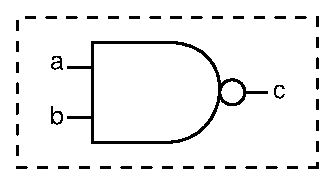
\includegraphics[scale=0.5]{nand2}
&
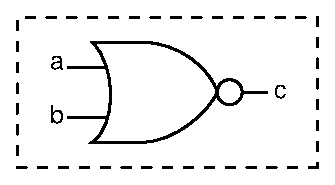
\includegraphics[scale=0.5]{nor2}
\\
\begin{minipage}[b]{2.5in}
\begin{ocamllisting}
class nand2 =
object
   inherit two_input_gate
   method compute_value = not (a && b)
end
\end{ocamllisting}
\end{minipage}
&
\begin{minipage}[b]{2.5in}
\begin{ocamllisting}
class nor2 =
object
   inherit two_input_gate
   method compute_value = not (a || b)
end
\end{ocamllisting}
\end{minipage}
\end{tabular}
\end{center}
%
\begin{enumerate}
\item 
Fill in the definitions of the methods \hbox{\lstinline/connect_input_a/} and \hbox{\lstinline/connect_input_b/}.

\begin{answer}\ifanswers
For the methods \hbox{\lstinline/connect_input_a/} we need to construct a terminal object
that performs the appropriate action.
\begin{ocaml}
   method connect_input_a (wire : wire) =
       wire#add_terminal (object method set x = self#set_input_a x end)
\end{ocaml}
\fi\end{answer}

\item
Define a class \hbox{\lstinline/three_input_gate/} (for gates with three inputs) by inheriting
from \hbox{\lstinline/two_input_gate/}.
\begin{answer}\ifanswers
\begin{ocaml}
class three_input_gate =
object
   inherit two_input_gate
   val mutable c = false
   method private set_input_c x = c <- x; self#set_output
   method connect_input_c (wire : wire) =
       wire#add_terminal (object method set x = self#set_input_c x end)
\end{ocaml}
\fi\end{answer}
   
\item
Would the definition be simpler if the type \hbox{\lstinline/terminal/} were a function instead of an
object (where \hbox{\lstinline/type terminal = bool -> unit/})?

\begin{answer}\ifanswers
It would be slightly simpler because the input terminal could be set without the intermediate terminal object.
The connect methods would have the following form.

\begin{ocaml}
   method connect_input_a (wire : wire) =
      wire#add_terminal self#set_input_a
\end{ocaml}
\fi\end{answer}

\item
What is the purpose of the conditional \hbox{\lstinline/if x <> value then $\cdots$/} in the class \hbox{\lstinline/wire/}?

\begin{answer}\ifanswers
The conditional prevents activity from propagating if it does not change the circuit values.
It also means that the simulation will terminate, even for cyclic circuits, if the circuit becomes quiescent.
\fi\end{answer}

\item
Write a program for the following circuit, called a \emph{SR latch}.
\begin{center}
\begin{tabular}{cc}
\begin{tabular}[b]{cc|c}
S & R & Action\\
\hline
0 & 0 & Keep state\\
0 & 1 & $Q = 0$\\
1 & 0 & $Q = 1$\\
1 & 1 & $Q = 0, \overline{Q} = 0$\\
\\
\end{tabular}
&
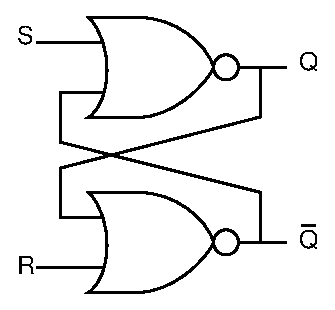
\includegraphics[scale=0.5]{latch}
\end{tabular}
\end{center}

\begin{answer}\ifanswers
\begin{ocaml}
let gate1 = new nor2;;
let gate2 = new nor2;;
let wire1 = new wire;;
let wire2 = new wire;;
gate1#connect_output wire1;;
gate2#connect_output wire2;;
gate1#connect_input_b wire2;;
gate2#connect_input_a wire1;;
\end{ocaml}
\fi\end{answer}
\end{enumerate}
\end{exercise}
   
\begin{exercise}{event-driven-simulator}
The simulator in Exercise~\ref{exercise:circuit-simulation}
has a problem with some cyclic circuits.  For example, the following circuit,
called a \emph{ring oscillator}, oscillates indefinitely, overflowing the stack during simulation.

\begin{center}
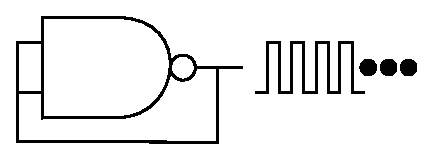
\includegraphics[scale=0.5]{ring}
\end{center}
%
The simulation can be executed in constant stack space by implementing an \emph{event-driven
simulator}.  In the circuit context, an \emph{event} occurs whenever the value on a terminal is set.
An event-driven simulator uses a scheduler to manage events.  When the value of a terminal is set,
the terminal is scheduled, but not executed yet.  When scheduled, the terminal is removed from the
scheduling queue and executed.

Define an event driven simulator by implementing a scheduler.  You can use a scheduling policy of
your choice, but it should be fair, meaning that if a terminal is scheduled, it will eventually be
executed.  

The scheduler should include a method \hbox{\lstinline/main : unit/} that runs until there are no more
events (perhaps forever).  The type \hbox{\lstinline/terminal/} should be defined as follows.
The method \hbox{\lstinline/set/} schedules the terminal, and the method \hbox{\lstinline/execute/} executes it.

\begin{ocaml}
type terminal = < set : bool -> unit; execute : unit >
\end{ocaml}

\begin{answer}\ifanswers
The scheduling queue can be implemented using the \hbox{\lstinline/Queue/} standard library.
This will use a FIFO policy, which is fair.

The scheduler has two methods.  The method \hbox{\lstinline/main/} runs the simulation until the
queue is empty.  The method \hbox{\lstinline/connect_input/} takes a wire and a function, creates
a terminal object, and add the object to the wire.  When the terminal is set, it gets
added to the scheduling queue.  Note that the field \hbox{\lstinline/event_queue/} is accessible
in the inner terminal object.

\begin{ocaml}
type terminal = < set : bool -> unit; execute : unit >

class scheduler =
object (self : 'self)
   val event_queue : terminal Queue.t = Queue.create ()

   method main =
       while not (Queue.is_empty event_queue) do
          (Queue.take event_queue)#execute
       done
   method connect_input (wire : wire) (f : bool -> unit) =
      let term =
         object (term_self)
            val mutable value = false
            method set x =
               value <- x;
               Queue.add term_self event_queue
            method execute = f value
         end
      in
      wire#add_terminal term
end;;

let the_scheduler = new scheduler;;
\end{ocaml}
%
The only other change to the simulation is to the methods \hbox{\lstinline/connect_input_?/}.

\begin{ocaml}
class virtual two_input_gate =
object (self : 'self)
   inherit gate
   val mutable a = false
   val mutable b = false
   method private set_input_a x = a <- x; self#set_output
   method private set_input_b x = b <- x; self#set_output
   method connect_input_a (wire : wire) =
      the_scheduler#connect_input wire self#set_input_a
   method connect_input_b (wire : wire) =
      the_scheduler#connect_input wire self#set_input_b
end
\end{ocaml}
\fi\end{answer}
\end{exercise}

% -*-
% Local Variables:
% Mode: LaTeX
% fill-column: 100
% TeX-master: "paper"
% TeX-command-default: "LaTeX/dvips Interactive"
% End:
% -*-
% vim:tw=100:fo=tcq:
